% Created 2020-07-13 lun 11:54
% Intended LaTeX compiler: pdflatex
\documentclass[presentation,aspectratio=1610]{beamer}
\usepackage[utf8]{inputenc}
\usepackage[T1]{fontenc}
\usepackage{graphicx}
\usepackage{grffile}
\usepackage{longtable}
\usepackage{wrapfig}
\usepackage{rotating}
\usepackage[normalem]{ulem}
\usepackage{amsmath}
\usepackage{textcomp}
\usepackage{amssymb}
\usepackage{capt-of}
\usepackage{hyperref}
\usepackage{khpreamble}
\usepackage{amssymb}
\DeclareMathOperator{\shift}{q}
\DeclareMathOperator{\diff}{p}
\usepgfplotslibrary{groupplots}
\usetheme{default}
\author{Kjartan Halvorsen}
\date{2020-07-13}
\title{Control Computarizado - Sintonización de PID}
\hypersetup{
 pdfauthor={Kjartan Halvorsen},
 pdftitle={Control Computarizado - Sintonización de PID},
 pdfkeywords={},
 pdfsubject={},
 pdfcreator={Emacs 26.3 (Org mode 9.3.6)}, 
 pdflang={English}}
\begin{document}

\maketitle


\section{Retroalimentación - Primer examen parcial}
\label{sec:orgf73edad}

\begin{frame}[label={sec:org67a4c4e}]{Retroalimentación - Primer examen parcial}
\begin{block}{Varias respuestas muy buenas}
\end{block}
\begin{block}{A mejorar}
\begin{itemize}
\item Profesor: Dar instrucciones más claras
\item Estudiantes: Leer bien las instrucciones
\end{itemize}
\end{block}
\end{frame}

\begin{frame}[label={sec:orgbfbe734}]{Retroalimentación - Primer examen parcial}
\[ \mathrm{e}^x = -1 \]
\[ x = \ln (-1) = ? \]
\end{frame}

\begin{frame}[label={sec:orgb22cec3}]{Retroalimentación - Primer examen parcial}
\[ \mathrm{e}^{i\pi} = -1 \]
\[ \ln (-1) = i\pi \]
\end{frame}

\begin{frame}[label={sec:org6a1c5c3}]{Retroalimentación - Primer examen parcial}
Respuesta al escalón de un motor DC
\begin{center}
  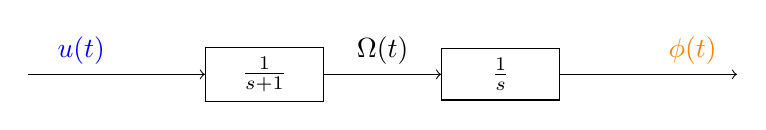
\begin{tikzpicture}[node distance=22mm, block/.style={rectangle, draw, minimum width=15mm}, sumnode/.style={circle, draw, inner sep=2pt}]

    \node[coordinate] (input) {};
    \node[block, right of=input, node distance=30mm] (plant)  {$\frac{1}{s+1}$};
    \node[block, right of=plant, node distance=30mm] (int) {$\frac{1}{s}$};
    \node[coordinate, right of=int, node distance=30mm] (output) {};

    \draw[->] (input) -- node[above, pos=0.3] {\textcolor{blue}{$u(t)$}} (plant);
    \draw[->] (plant) -- node[above,] {$\Omega(t)$} (int);
    \draw[->] (int) -- node[above, near end] {\textcolor{orange}{$\phi(t)$}} (output);
  \end{tikzpicture}
\end{center}
Cuál es el respuesto al escalón correcto del sistema?

\begin{center}
  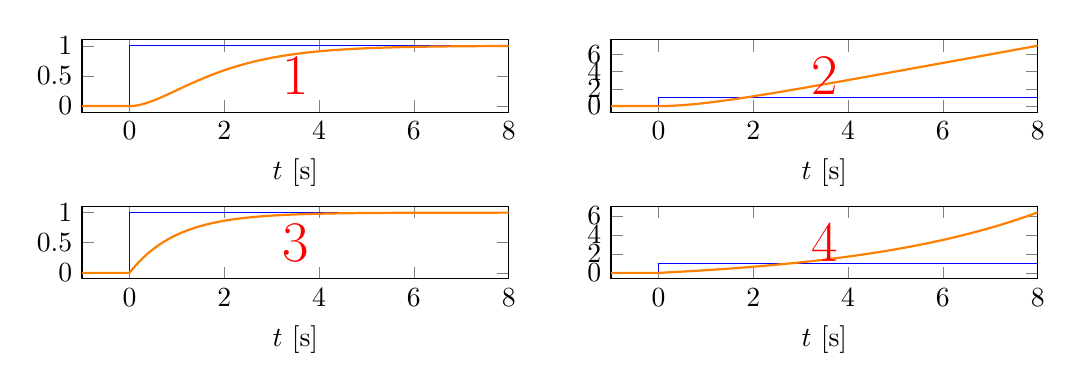
\begin{tikzpicture}
\begin{groupplot}[group style={group size=2 by 2, vertical sep=1.2cm, horizontal sep=1.3cm},
     width=7cm,
     height=2.5cm,
     xlabel={$t$ [s]},
     %ylabel={$y(t)$},
     xmin=-1,
     xmax=8,
     %ytick = \empty,
     %xtick = \empty,
     domain=-1:10,
     samples=400,
     variable=t,
     ]

     \nextgroupplot[]
     \addplot[blue, no marks] coordinates {(-1,0) (0,0) (0,1) (10,1)};
     \addplot[orange, thick,   no marks, smooth, ] { (t>0)*(-1 +exp(t) -t)*exp(-t) };

     \nextgroupplot[]
     \addplot[blue, no marks] coordinates {(-1,0) (0,0) (0,1) (10,1)};
     \addplot[orange, thick,   no marks, smooth, ] { (t>0)*(t + exp(-t) - 1) };

     \nextgroupplot[]
     \addplot[blue, no marks] coordinates {(-1,0) (0,0) (0,1) (10,1)};
     \addplot[orange, thick,   no marks, smooth, ] { (t>0)*(1 -exp(-t)) };

     \nextgroupplot[]
     \addplot[blue, no marks] coordinates {(-1,0) (0,0) (0,1) (10,1)};
     \addplot[orange, thick,   no marks, smooth, ] { (t>0)*(-1 +exp(t/4)) };

   \end{groupplot}

  \node[red] at (group c1r1.center) {\huge 1};
  \node[red] at (group c2r1.center) {\huge 2};
  \node[red] at (group c1r2.center) {\huge 3};
  \node[red] at (group c2r2.center) {\huge 4};
 \end{tikzpicture}
\end{center}
\end{frame}
\begin{frame}[label={sec:org86f6955}]{Retroalimentación - Primer examen parcial}
Problema 1
\[H_1(z) = \frac{0.035(z+0.88)}{(z-1)(z-0.67)}, \qquad h=0.2\]
Polos en 
\begin{align*}
z = 1  \quad &\Longrightleftarrow \quad s = \frac{\ln 1}{h} = 0 \\
z = 0.67  \quad &\Longrightleftarrow \quad s = \frac{\ln 0.67}{h} = -2.0 \\
\end{align*}

El polo en \(z=1\) está ubicado justamente \alert{sobre el circulo unitario} y no en el interior. El sistema \alert{no es estable}.
\end{frame}

\section{PID - repetición}
\label{sec:org2c6e6a5}

\begin{frame}[label={sec:org052778d}]{PID - repetición}
\end{frame}
\begin{frame}[label={sec:org60fd34b}]{PID con accción derivada sobre la variable de proceso}
\begin{center}
  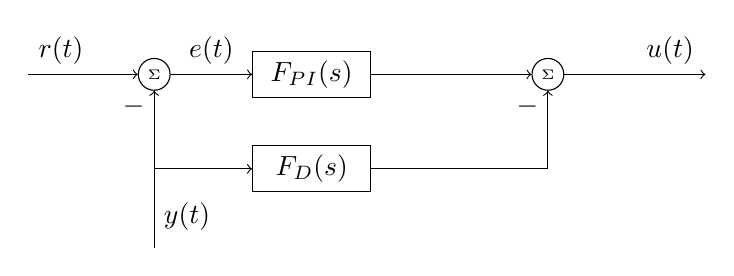
\begin{tikzpicture}[node distance=22mm, block/.style={rectangle, draw, minimum width=15mm}, sumnode/.style={circle, draw, inner sep=2pt}]

    \node[coordinate] (input) {};
    \node[sumnode, right of=input, node distance=16mm] (sum) {\tiny $\Sigma$};
    \node[block, right of=sum, node distance=20mm] (pi)  {$F_{PI}(s)$};
    \node[block, below of=pi, node distance=12mm] (dd)  {$F_{D}(s)$};
    \node[sumnode, right of=pi, node distance=30mm] (sum2) {\tiny $\Sigma$};
    \node[coordinate, below of=sum, node distance=22mm] (yy) {};
    \node[coordinate, right of=sum2, node distance=20mm] (output) {};

    \draw[->] (input) -- node[above, pos=0.3] {$r(t)$} (sum);
    \draw[->] (sum) -- node[above] {$e(t)$} (pi);
    \draw[->] (sum2) -- node[above, near end] {$u(t)$} (output);
    \draw[->] (yy) -- node[right, pos=0.2] {$y(t)$} node[pos=0.9, left] {$-$} (sum);
    \draw[->] (pi) -- node[above, near end] {} (sum2);
    \draw[->] (dd) -| node[left, pos=0.9] {$-$} (sum2);
    \draw[->] (yy) |- (dd);

  \end{tikzpicture}
\end{center}

\[ U(s) = \underbrace{K_c\left( 1 + \frac{1}{T_i s} \right)}_{F_{PI}(s)} E(s) - \underbrace{\frac{T_d s}{\frac{T_d}{N} s + 1}}_{F_{D}}Y(s)\]
\end{frame}

\section{Sintonización de PID}
\label{sec:org9641e83}
\begin{frame}[label={sec:orgc0823db}]{Sintonización de un PID}
\alert{El idéa} En forma experimental obtener unos pocos valores que capturan la dinámica del proceso. Usar una tabla predefinida para obtener las ganancias del PID dado estos valores.

Hay varios métodos. Ver el libro de texto y referencias incluidas.
\end{frame}

\begin{frame}[label={sec:org7a9d1cb}]{Sintonización de un PID - método de Smith \& Corripio}
Asuminedo modelo de proceso de primer orden con constante de tiempo \(T\) y retraso \(\tau\)
\[  \quad Y(s) = \frac{K\mathrm{e}^{-s\tau}}{sT + 1}U(s) \quad \overset{U(s) = \frac{u_f}{s}}{\Longrightarrow} \quad y(t) = u_f K\big( 1 - \mathrm{e}^{-\frac{t-\tau}{T}}\big)u_s(t-\tau)\]
\def\Tcnst{3}
\def\tdelay{0.6}
\def\ggain{2}
\def\uampl{0.8}
\pgfmathsetmacro{\yfinal}{\uampl*\ggain}
\pgfmathsetmacro{\yone}{0.283*\yfinal}
\pgfmathsetmacro{\ytwo}{0.632*\yfinal}
\pgfmathsetmacro{\tone}{\tdelay + \Tcnst/3}
\pgfmathsetmacro{\two}{\tdelay + \Tcnst}

\begin{center}
  \begin{tikzpicture}
    \begin{axis}[
    width=14cm,
    height=5cm,
    grid = both,
    xtick = {0, \tdelay, \tone, \two},
    xticklabels = {0, $\tau$, $\tau+\frac{T}{3}$, $\tau + T$},
    ytick = {0, \yone, \ytwo, \uampl, \yfinal},
    yticklabels = {0, $0.283y_{f}$, $0.632y_f$, $u_f$, $y_f$},
    xmin = -0.2,
    %minor y tick num=9,
    %minor x tick num=9,
    %every major grid/.style={red, opacity=0.5},
    xlabel = {$t$},
    ]
      \addplot [thick, green!50!black, no marks, domain=0:10, samples=100] {\uampl*\ggain*(x>\tdelay)*(1 - exp(-(x-\tdelay)/\Tcnst)} node [coordinate, pos=0.9, pin=-90:{$y(t)$}] {};
      \addplot [const plot, thick, blue!80!black, no marks, domain=-1:10, samples=100] coordinates {(-1,0) (0,0) (0,\uampl) (10,\uampl)} node [coordinate, pos=0.9, pin=-90:{$u(t)$}] {};
    \end{axis}
  \end{tikzpicture}
\end{center}

\[ y_f = \lim_{t\to\infty} y(t) = u_f K \quad \Rightarrow \quad K = \frac{y_f}{u_f}. \]
\end{frame}

\begin{frame}[label={sec:org2ccf1c0}]{Método de Smith \& Corripio - ejemplo}
\[  \quad Y(s) = \frac{K\mathrm{e}^{-s\tau}}{sT + 1}U(s) \quad \overset{U(s) = \frac{u_f}{s}}{\Longrightarrow} \quad y(t) = u_f K\big( 1 - \mathrm{e}^{-\frac{t-\tau}{T}}\big)u_s(t-\tau)\]
\def\Tcnst{2.1}
\def\tdelay{1}
\def\ggain{2}
\def\uampl{0.8}
\pgfmathsetmacro{\yfinal}{\uampl*\ggain}
\pgfmathsetmacro{\yone}{0.283*\yfinal}
\pgfmathsetmacro{\ytwo}{0.632*\yfinal}
\pgfmathsetmacro{\tone}{\tdelay + \Tcnst/3}
\pgfmathsetmacro{\two}{\tdelay + \Tcnst}

\begin{center}
  \begin{tikzpicture}
    \begin{axis}[
    width=12cm,
    height=4cm,
    grid = both,
    %xtick = {0, \tdelay, \tone, \two},
    %xticklabels = {0, $\tau$, $\tau+\frac{T}{3}$, $\tau + T$},
    %ytick = {0, \yone, \ytwo, \uampl, \yfinal},
    %yticklabels = {0, $0.283y_{f}$, $0.632y_f$, $u_f$, $y_f$},
    xmin = -0.2,
    minor y tick num=9,
    minor x tick num=9,
    every major grid/.style={red, opacity=0.5},
    %xlabel = {$t$},
    clip = false,
    ]
      \addplot [thick, green!50!black, smooth, no marks, domain=0:10, samples=16] {\uampl*\ggain*(x>\tdelay)*(1 - exp(-(x-\tdelay)/\Tcnst)} node [coordinate, pos=0.9, pin=-90:{$y(t)$}] {};
      \addplot [const plot, thick, blue!80!black, no marks, domain=-1:10, samples=100] coordinates {(-1,0) (0,0) (0,\uampl) (10,\uampl)} node [coordinate, pos=0.9, pin=-90:{$u(t)$}] {};
      \draw[thick, red, dashed] (axis cs: \tone, \yone) -- (axis cs: \tone, -0.45) node[below] {$t_1 = \tone = \tau + \frac{T}{3}$}; 
      \draw[thick, red, dashed] (axis cs: \tone, \yone) -- (axis cs: -1,\yone) node[left, anchor=east] {$0.283y_f = \yone$}; 
      \draw[thick, orange, dashed] (axis cs: \two, \ytwo) -- (axis cs: \two, -0.9) node[below] {$t_2 = \two = \tau + T$}; 
      \draw[thick, orange, dashed] (axis cs: \two, \ytwo) -- (axis cs: -1, \ytwo, -0.9) node[left, anchor=east] {$0.632y_f = \ytwo$}; 
      \draw[thick, green!70!black, dashed] (axis cs: 10, \yfinal) -- (axis cs: -1, \yfinal, -0.9) node[left, anchor=east] {$y_f = \yfinal$}; 
      \draw[blue!70!black, dashed] (axis cs: 0, \uampl) -- (axis cs: -1, \uampl, -0.9) node[left, anchor=east] {$u_f = \uampl$}; 
    \end{axis}
  \end{tikzpicture}
\end{center}
\[ \begin{cases} \tone = \tau + \frac{T}{3}\\ \two = \tau + T \end{cases} \quad \Rightarrow \quad \begin{cases} \tau = \tdelay \\ T = \Tcnst \end{cases}, \qquad  K = \frac{y_f}{u_f} = \frac{\yfinal}{\uampl} = \ggain \]
\end{frame}

\begin{frame}[label={sec:org003c39a}]{Método de Smith \& Corripio - ejercicio}
\alert{Actividad} En grupos de dos: Comparte pantalla con esta diapositiva. Marca \(y_f\), \(0.632y_f\), \(0.283y_f\), \(u_f\), \(t_1\) y \(t_2\). Determina los parametros del modelo de primer orden con retraso.

\def\uampl{0.5}
\def\ttdelay{0.3}
\def\TTcnst{1.6}
\def\ggain{3}

\pgfmathsetmacro{\yfinal}{\uampl*\ggain}
\pgfmathsetmacro{\yone}{0.283*\yfinal}
\pgfmathsetmacro{\ytwo}{0.632*\yfinal}
\pgfmathsetmacro{\tone}{\tdelay + \Tcnst/3}
\pgfmathsetmacro{\two}{\tdelay + \Tcnst}


\begin{center}
  \begin{tikzpicture}
    \begin{axis}[
    width=13cm,
    height=6cm,
    grid = both,
    minor y tick num=9,
    minor x tick num=9,
    every major grid/.style={red, opacity=0.5},
    xlabel = {$t$},
    xmin = -1,
    ]
      \addplot [thick, green!50!black, no marks, domain=0:10, smooth, samples=16] {\uampl*\ggain*(x>\ttdelay)*(1 - (1+(x-\ttdelay)/\TTcnst)*exp(-(x-\ttdelay)/\TTcnst))} node [coordinate, pos=0.9, pin=-90:{$y(t)$}] {};
      \addplot [const plot, thick, blue!80!black, no marks, domain=-1:10, samples=100] coordinates {(-1,0) (0,0) (0,\uampl) (10,\uampl)} node [coordinate, pos=0.9, pin=-90:{$u(t)$}] {};
    \end{axis}
  \end{tikzpicture}
\end{center}
\end{frame}

\begin{frame}[label={sec:orgf08bb50}]{Método de Smith \& Corripio - solución}
\end{frame}
\begin{frame}[label={sec:org4f80fc6}]{Método de Smith \& Corripio - solución}
\def\uampl{0.5}
\def\ttdelay{0.3}
\def\TTcnst{1.6}
\def\ggain{3}
\def\tdelay{1.125} % Resulting from method
\def\Tcnst{2.625} % Resulting from method

\pgfmathsetmacro{\yfinal}{\uampl*\ggain}
\pgfmathsetmacro{\yone}{0.283*\yfinal}
\pgfmathsetmacro{\ytwo}{0.632*\yfinal}
\pgfmathsetmacro{\tone}{2}
\pgfmathsetmacro{\two}{3.75}


\begin{center}
  \begin{tikzpicture}
    \begin{axis}[
    width=12cm,
    height=5cm,
    grid = both,
    minor y tick num=9,
    minor x tick num=9,
    every major grid/.style={red, opacity=0.5},
    xlabel = {$t$},
    xmin = -1,
    clip=false,
    ]
      \addplot [thick, green!50!black, no marks, domain=0:10, smooth, samples=16] {\uampl*\ggain*(x>\ttdelay)*(1 - (1+(x-\ttdelay)/\TTcnst)*exp(-(x-\ttdelay)/\TTcnst))} node [coordinate, pos=0.9, pin=-90:{$y(t)$}] {};
      \addplot [const plot, thick, blue!80!black, no marks, domain=-1:10, samples=100] coordinates {(-1,0) (0,0) (0,\uampl) (10,\uampl)} node [coordinate, pos=0.9, pin=-90:{$u(t)$}] {};
      \draw[thick, red, dashed] (axis cs: \tone, \yone) -- (axis cs: \tone, -0.45) node[below] {$t_1 = \tone = \tau + \frac{T}{3}$}; 
      \draw[thick, red, dashed] (axis cs: \tone, \yone) -- (axis cs: -2,\yone) node[left, anchor=east] {$0.283y_f = \yone$}; 
      \draw[thick, orange, dashed] (axis cs: \two, \ytwo) -- (axis cs: \two, -0.9) node[below] {$t_2 = \two = \tau + T$}; 
      \draw[thick, orange, dashed] (axis cs: \two, \ytwo) -- (axis cs: -2, \ytwo, -0.9) node[left, anchor=east] {$0.632y_f = \ytwo$}; 
      \draw[thick, green!60!black, dashed] (axis cs: 10, \yfinal) -- (axis cs: -2, \yfinal) node[left, anchor=east] {$y_f = \yfinal$}; 
      \draw[blue!70!black, dashed] (axis cs: 10, \uampl) -- (axis cs: 10.2, \uampl, -0.9) node[above] {$u_f = \uampl$}; 

    \end{axis}
  \end{tikzpicture}
\end{center}
\[ \begin{cases} \tone = \tau + \frac{T}{3}\\ \two = \tau + T \end{cases} \quad \Rightarrow \quad \begin{cases} \tau = 1.125 \\ T = 2.625 \end{cases}, \qquad  K = \frac{y_f}{u_f} = \frac{\yfinal}{\uampl} = \ggain \]
\end{frame}
\begin{frame}[label={sec:org9e8a1ec}]{Método de Smith \& Corripio - solución}
\def\uampl{0.5}
\def\ttdelay{0.3}
\def\TTcnst{1.6}
\def\ggain{3}
\def\tdelay{1.125} % Resulting from method
\def\Tcnst{2.625} % Resulting from method

\pgfmathsetmacro{\yfinal}{\uampl*\ggain}
\pgfmathsetmacro{\yone}{0.283*\yfinal}
\pgfmathsetmacro{\ytwo}{0.632*\yfinal}
\pgfmathsetmacro{\tone}{2}
\pgfmathsetmacro{\two}{3.75}


\begin{center}
  \begin{tikzpicture}
    \begin{axis}[
    width=12cm,
    height=5.5cm,
    grid = both,
    minor y tick num=9,
    minor x tick num=9,
    every major grid/.style={red, opacity=0.5},
    xlabel = {$t$},
    xmin = -1,
    clip=false,
    ]
      \addplot [thick, green!50!black, no marks, domain=0:10, smooth, samples=16] {\uampl*\ggain*(x>\ttdelay)*(1 - (1+(x-\ttdelay)/\TTcnst)*exp(-(x-\ttdelay)/\TTcnst))} node [coordinate, pos=0.9, pin=-90:{$y(t)$}] {};
      \addplot [const plot, thick, blue!80!black, no marks, domain=-1:10, samples=100] coordinates {(-1,0) (0,0) (0,\uampl) (10,\uampl)} node [coordinate, pos=0.9, pin=-90:{$u(t)$}] {};
      \addplot [thick, olive!80!black, smooth, no marks, domain=0:10, samples=100] {\uampl*\ggain*(x>\tdelay)*(1 - exp(-(x-\tdelay)/\Tcnst)} node [coordinate, pos=0.6, pin=-90:{model}] {};
      \draw[thick, red, dashed] (axis cs: \tone, \yone) -- (axis cs: \tone, -0.45) node[below] {$t_1 = \tone = \tau + \frac{T}{3}$}; 
      \draw[thick, red, dashed] (axis cs: \tone, \yone) -- (axis cs: -2,\yone) node[left, anchor=east] {$0.283y_f = \yone$}; 
      \draw[thick, orange, dashed] (axis cs: \two, \ytwo) -- (axis cs: \two, -0.9) node[below] {$t_2 = \two = \tau + T$}; 
      \draw[thick, orange, dashed] (axis cs: \two, \ytwo) -- (axis cs: -2, \ytwo, -0.9) node[left, anchor=east] {$0.632y_f = \ytwo$}; 
      \draw[thick, green!60!black, dashed] (axis cs: 10, \yfinal) -- (axis cs: -2, \yfinal) node[left, anchor=east] {$y_f = \yfinal$}; 
      \draw[blue!70!black, dashed] (axis cs: 10, \uampl) -- (axis cs: 10.2, \uampl, -0.9) node[above] {$u_f = \uampl$}; 

    \end{axis}
  \end{tikzpicture}
\end{center}


\[ \text{\textcolor{olive}{Model:}} \qquad  \textcolor{olive}{G(s) = \ggain \frac{\mathrm{e}^{-\tdelay s}}{\Tcnst s + 1}} \]
\end{frame}

\begin{frame}[label={sec:org1b1027b}]{Método de Smith \& Corripio - Tabla de Ziegler-Nichols}
Dado el modelo 
\[ G(s) = K \frac{\mathrm{e}^{-s\tau}}{sT + 1} \]
Elige los parametros PID según la tabla de Ziegler y Nichols (1943)
   \begin{center}
   \setlength{\tabcolsep}{20pt}
   \renewcommand{\arraystretch}{1.5}
   \begin{tabular}{llll}
   Controlador & \(K_c\) & \(T_i\) & \(T_d\)\\
  \hline\hline
  P & \(\frac{T}{\tau K}\) &  & \\
  PI & \(\frac{0.9T}{\tau K}\) & \(\frac{\tau}{0.3}\) & \\
  PID & \(\frac{1.2T}{\tau K}\) & \(2\tau\) & \(\frac{\tau}{2}\)\\
  \hline
\end{tabular}
\end{center}

Funciona bien cuando \[0.1 < \frac{\tau}{T} < 0.6.\]
\end{frame}


\begin{frame}[label={sec:orgd6f9fbf}]{Tabla de  Ziegler-Nichols - ejemplo}
\[ G(s) = K \frac{\mathrm{e}^{-s\tau}}{sT + 1} = 2 \frac{\mathrm{e}^{-s}}{s2.1 + 1} \]
   \begin{center}
   \setlength{\tabcolsep}{20pt}
   \renewcommand{\arraystretch}{1.5}
   \begin{tabular}{llll}
   Controlador & \(K_c\) & \(T_i\) & \(T_d\)\\
  \hline\hline
  P & \(\frac{T}{\tau K} = \frac{2.1}{1 \cdot 2} = 1.05\) &  & \\
  PI & \(\frac{0.9T}{\tau K} = \frac{0.9\cdot 2.1}{2}= 0.945\) & \(\frac{\tau}{0.3} = \frac{1}{3} \) & \\
  PID & \(\frac{1.2T}{\tau K} = 1.26 \) & \(2\tau=2\) & \(\frac{\tau}{2}=\frac{1}{2}\)\\
  \hline
\end{tabular}
\end{center}
Regla de control (PID completo, \(N=10\)):
\[ U(s) = K_c\left( 1 + \frac{1}{T_i s} \right) E(s) - \frac{T_d s}{\frac{T_d}{N} s + 1}Y(s)
           =  1.26\left( 1 + \frac{1}{2 s} \right) E(s) - \frac{0.5s}{\frac{0.5}{10} s + 1}Y(s)\]
\end{frame}


\begin{frame}[label={sec:orgbe56985}]{Tabla de  Ziegler-Nichols - ejercicio}
Determina los parametros del PID para el modelo del ejercicio anterior \(\tau = 1.125\), \(T = 2.625\).

\[ G(s) = K \frac{\mathrm{e}^{-s\tau}}{sT + 1} =  \qquad\qquad\qquad\qquad\qquad\qquad \]
   \begin{center}
   \setlength{\tabcolsep}{20pt}
   \renewcommand{\arraystretch}{1.5}
   \begin{tabular}{llll}
   Controlador & \(K_c\) & \(T_i\) & \(T_d\)\\
  \hline\hline
  P & \(\frac{T}{\tau K} = \) &  & \\
  PI & \(\frac{0.9T}{\tau K} = \) & \(\frac{\tau}{0.3} = \) & \\
  PID & \(\frac{1.2T}{\tau K} = \) & \(2\tau\) & \(\frac{\tau}{2}=\)\\
  \hline
\end{tabular}
\end{center}
Regla de control (PID completo, \(N=?\)):
\[ U(s) = K_c\left( 1 + \frac{1}{T_i s} \right) E(s) - \frac{T_d s}{\frac{T_d}{N} s + 1}Y(s)
           =  \qquad\qquad\qquad\qquad\qquad\qquad\quad\quad\]
\end{frame}



\section{Asignación de polos}
\label{sec:orgc203dd3}
\begin{frame}[label={sec:org1b62dd5}]{Asignación de polos - Un ejemplo}
\begin{center}
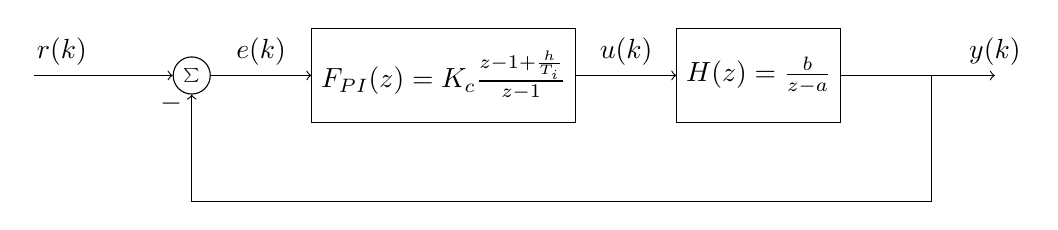
\begin{tikzpicture}
\tikzset{node distance=2cm, 
    block/.style={rectangle, draw, minimum height=12mm, minimum width=14mm},
    sumnode/.style={circle, draw, inner sep=2pt}        
}

  \node[coordinate] (input) {};
  \node[sumnode, right of=input, node distance=20mm] (sum) {\tiny $\sum$};
  \node[block, right of=sum, node distance=32mm] (PI) {$F_{PI}(z) = K_c\frac{z -1 + \frac{h}{T_i}}{z-1}$};
  \node[block,right of=PI, node distance=40mm] (plant) {$H(z) = \frac{b}{z-a}$};
  \node[coordinate, right of=plant, node distance=30mm] (output) {};
  \node[coordinate, right of=plant, node distance=22mm] (measure) {};
  \draw[->] (input) -- node[above, pos=0.2] {$r(k)$} (sum);
  \draw[->] (sum) -- node[above, ] {$e(k)$} (PI);
  \draw[->] (PI) -- node[above] {$u(k)$} (plant);
  \draw[->] (plant) -- node[at end, above] {$y(k)$} (output);
  \draw[->] (measure) -- ++(0,-16mm) -| (sum) node[left, pos=0.96] {$-$};
\end{tikzpicture}
\end{center}

\alert{Queremos un sistema de lazo cerrado criticalmente amortiguado con dos polos en \(z = \alpha, \quad 0 < \alpha < 1\)}
\end{frame}


\begin{frame}[label={sec:orgd5f97c7}]{Asignación de polos}
\begin{center}
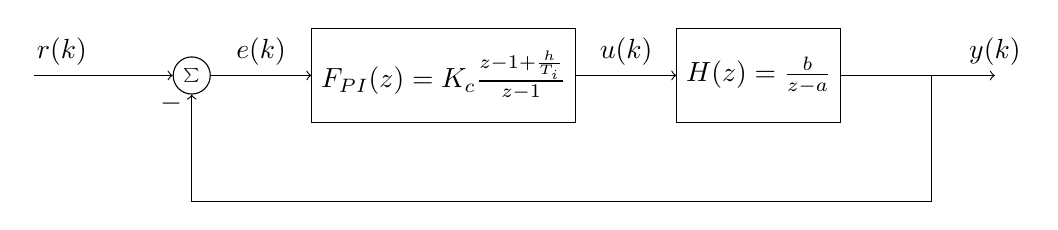
\begin{tikzpicture}
\tikzset{node distance=2cm, 
    block/.style={rectangle, draw, minimum height=12mm, minimum width=14mm},
    sumnode/.style={circle, draw, inner sep=2pt}        
}

  \node[coordinate] (input) {};
  \node[sumnode, right of=input, node distance=20mm] (sum) {\tiny $\sum$};
  \node[block, right of=sum, node distance=32mm] (PI) {$F_{PI}(z) = K_c\frac{z -1 + \frac{h}{T_i}}{z-1}$};
  \node[block,right of=PI, node distance=40mm] (plant) {$H(z) = \frac{b}{z-a}$};
  \node[coordinate, right of=plant, node distance=30mm] (output) {};
  \node[coordinate, right of=plant, node distance=22mm] (measure) {};
  \draw[->] (input) -- node[above, pos=0.2] {$r(k)$} (sum);
  \draw[->] (sum) -- node[above, ] {$e(k)$} (PI);
  \draw[->] (PI) -- node[above] {$u(k)$} (plant);
  \draw[->] (plant) -- node[at end, above] {$y(k)$} (output);
  \draw[->] (measure) -- ++(0,-16mm) -| (sum) node[left, pos=0.96] {$-$};
\end{tikzpicture}
\end{center}

\alert{Ecuación característica}
\begin{align*}
1 + H(z)F_{PI}(z) &= 0\\
(z-1)(z-a) + K_c b (z - 1 + h/T_i) &= 0
\end{align*}
\alert{Polinomio característico}
\[ \underbrace{(z-1)(z-a) + K_c b (z - 1 + h/T_i)}_{\text{parametrizado}} = \underbrace{(z-\alpha)^2}_{\text{deseado}}\]

\alert{¿Cómo podemos determinar los parametros del controlador, \(K_c\) y \(T_i\)?} 
\end{frame}

\begin{frame}[label={sec:org0c7f24a}]{Asignación de polos - Solución}
\begin{center}
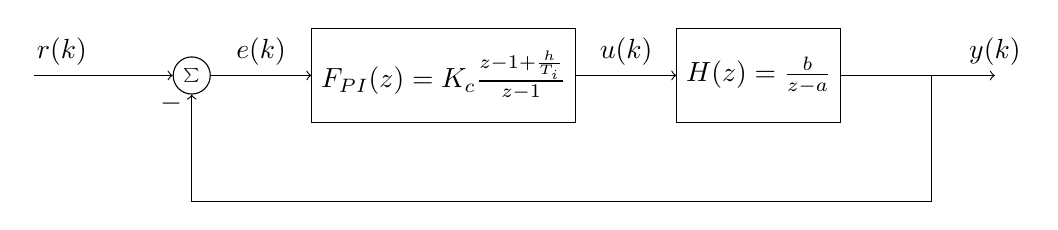
\begin{tikzpicture}
\tikzset{node distance=2cm, 
    block/.style={rectangle, draw, minimum height=12mm, minimum width=14mm},
    sumnode/.style={circle, draw, inner sep=2pt}        
}

  \node[coordinate] (input) {};
  \node[sumnode, right of=input, node distance=20mm] (sum) {\tiny $\sum$};
  \node[block, right of=sum, node distance=32mm] (PI) {$F_{PI}(z) = K_c\frac{z -1 + \frac{h}{T_i}}{z-1}$};
  \node[block,right of=PI, node distance=40mm] (plant) {$H(z) = \frac{b}{z-a}$};
  \node[coordinate, right of=plant, node distance=30mm] (output) {};
  \node[coordinate, right of=plant, node distance=22mm] (measure) {};
  \draw[->] (input) -- node[above, pos=0.2] {$r(k)$} (sum);
  \draw[->] (sum) -- node[above, ] {$e(k)$} (PI);
  \draw[->] (PI) -- node[above] {$u(k)$} (plant);
  \draw[->] (plant) -- node[at end, above] {$y(k)$} (output);
  \draw[->] (measure) -- ++(0,-16mm) -| (sum) node[left, pos=0.96] {$-$};
\end{tikzpicture}
\end{center}
\alert{Polinomio característico}
\[ \underbrace{z^2 - (1+a -K_cb)z + K_cb(h/T_i - 1) + a}_{\text{parametrizado}} = \underbrace{z^2 -2\alpha z + \alpha^2}_{\text{deseado}}\]

\begin{align*}
1 + a - K_c b &= 2\alpha \quad \Rightarrow \quad K_c = \frac{1+a-2\alpha}{b}\\
K_cb(h/T_i - 1) + a &= \alpha^2 \quad \Rightarrow \quad \frac{1}{T_i} = \frac{1}{h}\left(1 + \frac{\alpha^2-a}{K_c b}\right) = \frac{1}{h} \left( \frac{(\alpha-1)^2}{1 + a - 2\alpha}\right) 
\end{align*}
\end{frame}


\begin{frame}[label={sec:org0d97078}]{Asignación de polos}
Ligas

\href{https://mybinder.org/v2/gh/kjartan-at-tec/mr2007-computerized-control/master?filepath=.\%2Fapproximating-cont-controller\%2Fnotebooks\%2FPole-placement-PI-controller-example.ipynb}{Solución en mybinder}

\href{https://github.com/kjartan-at-tec/mr2007-computerized-control/blob/master/approximating-cont-controller/notebooks/Pole-placement-PI-controller-example.ipynb}{Solución en github}
\end{frame}
\end{document}